\section{Systemtest med kendt input}
I dette afsnit vil det samlede system blive testet, så det er muligt at se, om systemet behandler dette input, som det forventes. På baggrund af disse målinger er det muligt at konkludere, om systemet virker. 

\subsection{Beskrivelse}
For at teste det samlede system med et kendt input benyttes en funktionsgenerator, så der kan genereres et sinussignal på $500~Hz$ med en peak-peak-amplitude på $4~mV$. På denne måde ses effekten af systemets blokke, når de er sammensat, da input-signalet og outputtet fra EMG-algoritmen herved kan sammenlignes i MATLAB. Sinussignalet er lavpasfiltreret og sammenlignes med et filtreret EMG-signal, da sinussignalets frekvens og peak-peak-amplitude er nær ved, hvad der kunne forventes af det filtrerede EMG-signal. Systemet testes ved at måle systemets output i 10 sekunder, mens der sende et sinussignal ind i lavpasfilteret og fungere som et input.
 
 
 
mens spænding, der almindeligvis kommer ind via accelerometrene, varieres således, at den overskrider de spændinger, der tilsvarer $90-180^{\circ}$. 
Dermed kan udregnes et forventet output til det valgte input, hvilke kan sammenholdes med det reelle output. Afvigelsen herfra vil herefter kunne beregnes. 
 
\subsection{Resultater af test}
Fra testen plottes og visualiseres systemets input og output i MATLAB, hvilket fremgår af \autoref{fig:test_kendtinput}. 

\begin{figure}[H]
\centering
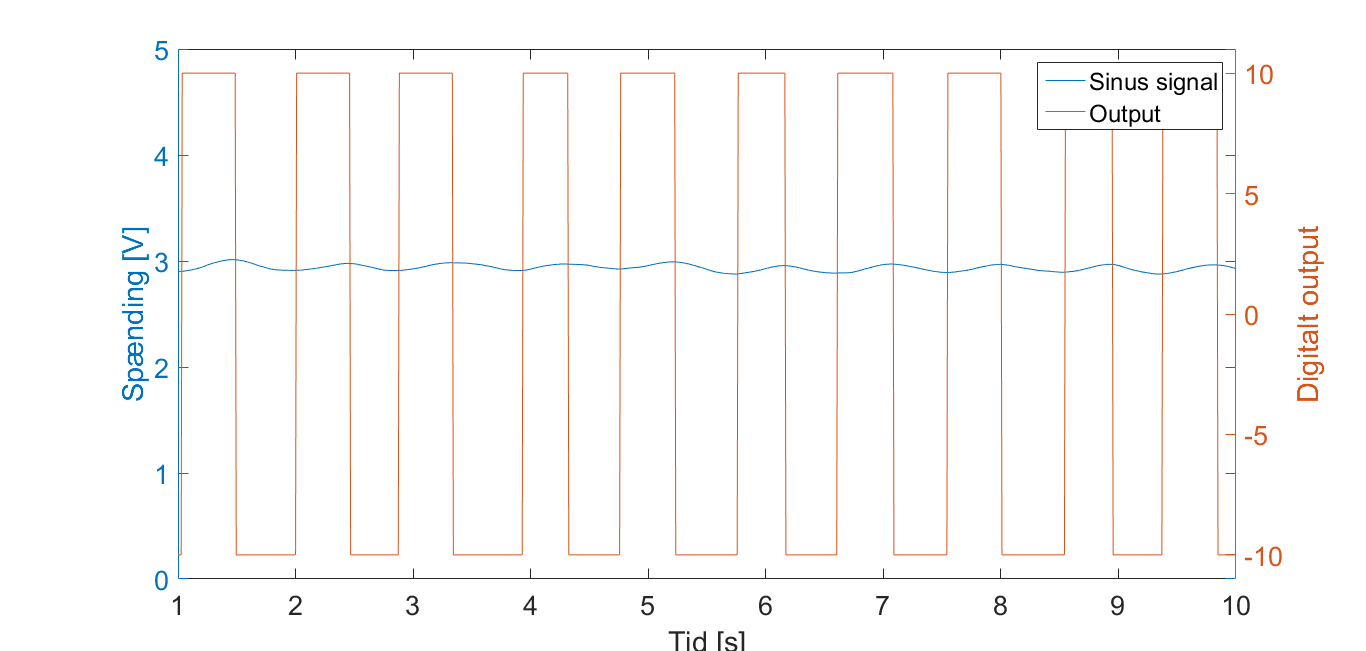
\includegraphics[width=0.4\textwidth]{figures/kontrol_test_sinus.jpg}
\caption{Den blå graf illustrerer det filtrede sinussignal, der er EMG-algoitmens input, mens den røde grad illustrerer om inputsignalet er stigende eller faldende ved at udsende et signal på henholdsvis $-10~V$ eller $10~V$.}
\label{fig:test_kendtinput}
\end{figure}

På baggrund af målingerne for \autoref{fig:test_kendtinput} findes lokale maksima- og minimapunkter. For at kunne udregne forsinkelsen sammenlignes forskellen mellem de lokale ekstrema, hvor der undersøges hvornår outputtet skifter spænding, altså differensen mellem lokale ekstrema og skift i outputspænding. Resultaterne for dette fremgår af \autoref{tab:sinus_ekstrema}.


\begin{table}[H]
\centering
\begin{tabular}{|c|c|c|}
\hline
\textbf{Ekstrema {[}s{]}} & \textbf{Output-skift {[}s{]}} & \textbf{Forsinkelse {[}s{]}} \\ \hline
3,0132                    & 2,8778                        & 0,1354                       \\ \hline
2,9922                    & 2,8859                        & 0,1063                       \\ \hline
2,9842                    & 2,8907                        & 0,0935                       \\ \hline
2,9777                    & 2,8939                        & 0,0838                       \\ \hline
2,9713                    & 2,9020                        & 0,0693                       \\ \hline
2,9713                    & 2,9101                        & 0,0612                       \\ \hline
2,9681                    & 2,9101                        & 0,0580                       \\ \hline
2,9681                    & 2,9117                        & 0,0564                       \\ \hline
2,9632                    & 2,9246                        & 0,0386                       \\ \hline
2,9568                    & 2,9278                        & 0,0290                       \\ \hline
\end{tabular}
\caption{Målt ekstrema, output-skift og differensen mellem disse, som fremgår som forsinkelse}
\label{tab:sinus_ekstrema}
\end{table}

Af \autoref{tab:sinus_ekstrema} fremgår det, at forsinkelsen fra inputsignalet registreres som en ændring  i output-signalet og er mellem $0,0290~s$ og $0,1354~s$. Ud fra dette er den gennemsnitlige forsinkelse beregnet til at være $0,07315~s$, hvilket svarer til omkring $73~ms$. 


\subsection{Konklusion}
.....